\documentclass{beamer}

\usepackage{color}
\usepackage{graphicx}
\usepackage{geometry}
\usepackage{url}
\usepackage{pgfpages}
\usepackage{color}
\usepackage{ifthen}
\usetheme{Berlin}
\usecolortheme{ufrn}

\title[Turks in Germany]{Ausl{\"a}nder}
\date{\today}
\author{Brennan W. Fieck}
\institute{LAIS 418 - Narrating the Notion}

\setbeamertemplate{headline}
{%
	\begin{beamercolorbox}[colsep=1.5pt]{upper separation line head}
	\end{beamercolorbox}
	\begin{beamercolorbox}{section in head/foot}
		\vskip2pt\insertnavigation{paperwidth}\vskip2pt
	\end{beamercolorbox}%
	\begin{beamercolorbox}[colsep=1.5pt]{lower separation line head}
	\end{beamercolorbox}
}

\begin{document}
\frame{\titlepage}
\section{}
\begin{frame}{Summary}
	\tableofcontents
\end{frame}

\section{Early Incursions}
\begin{frame}{Early Incursions}
	\begin{columns}
		\column{0.6\textwidth}
			\begin{enumerate}
				\item Sieges of Vienna (1529, 1683)
				\item Great Turkish War (1683-1699)
				\item Prussian Soldiers (mid 1700's)
			\end{enumerate}
		\column{0.4\textwidth}
			\vcenter
			\begin{figure}[ht]
				\centering
				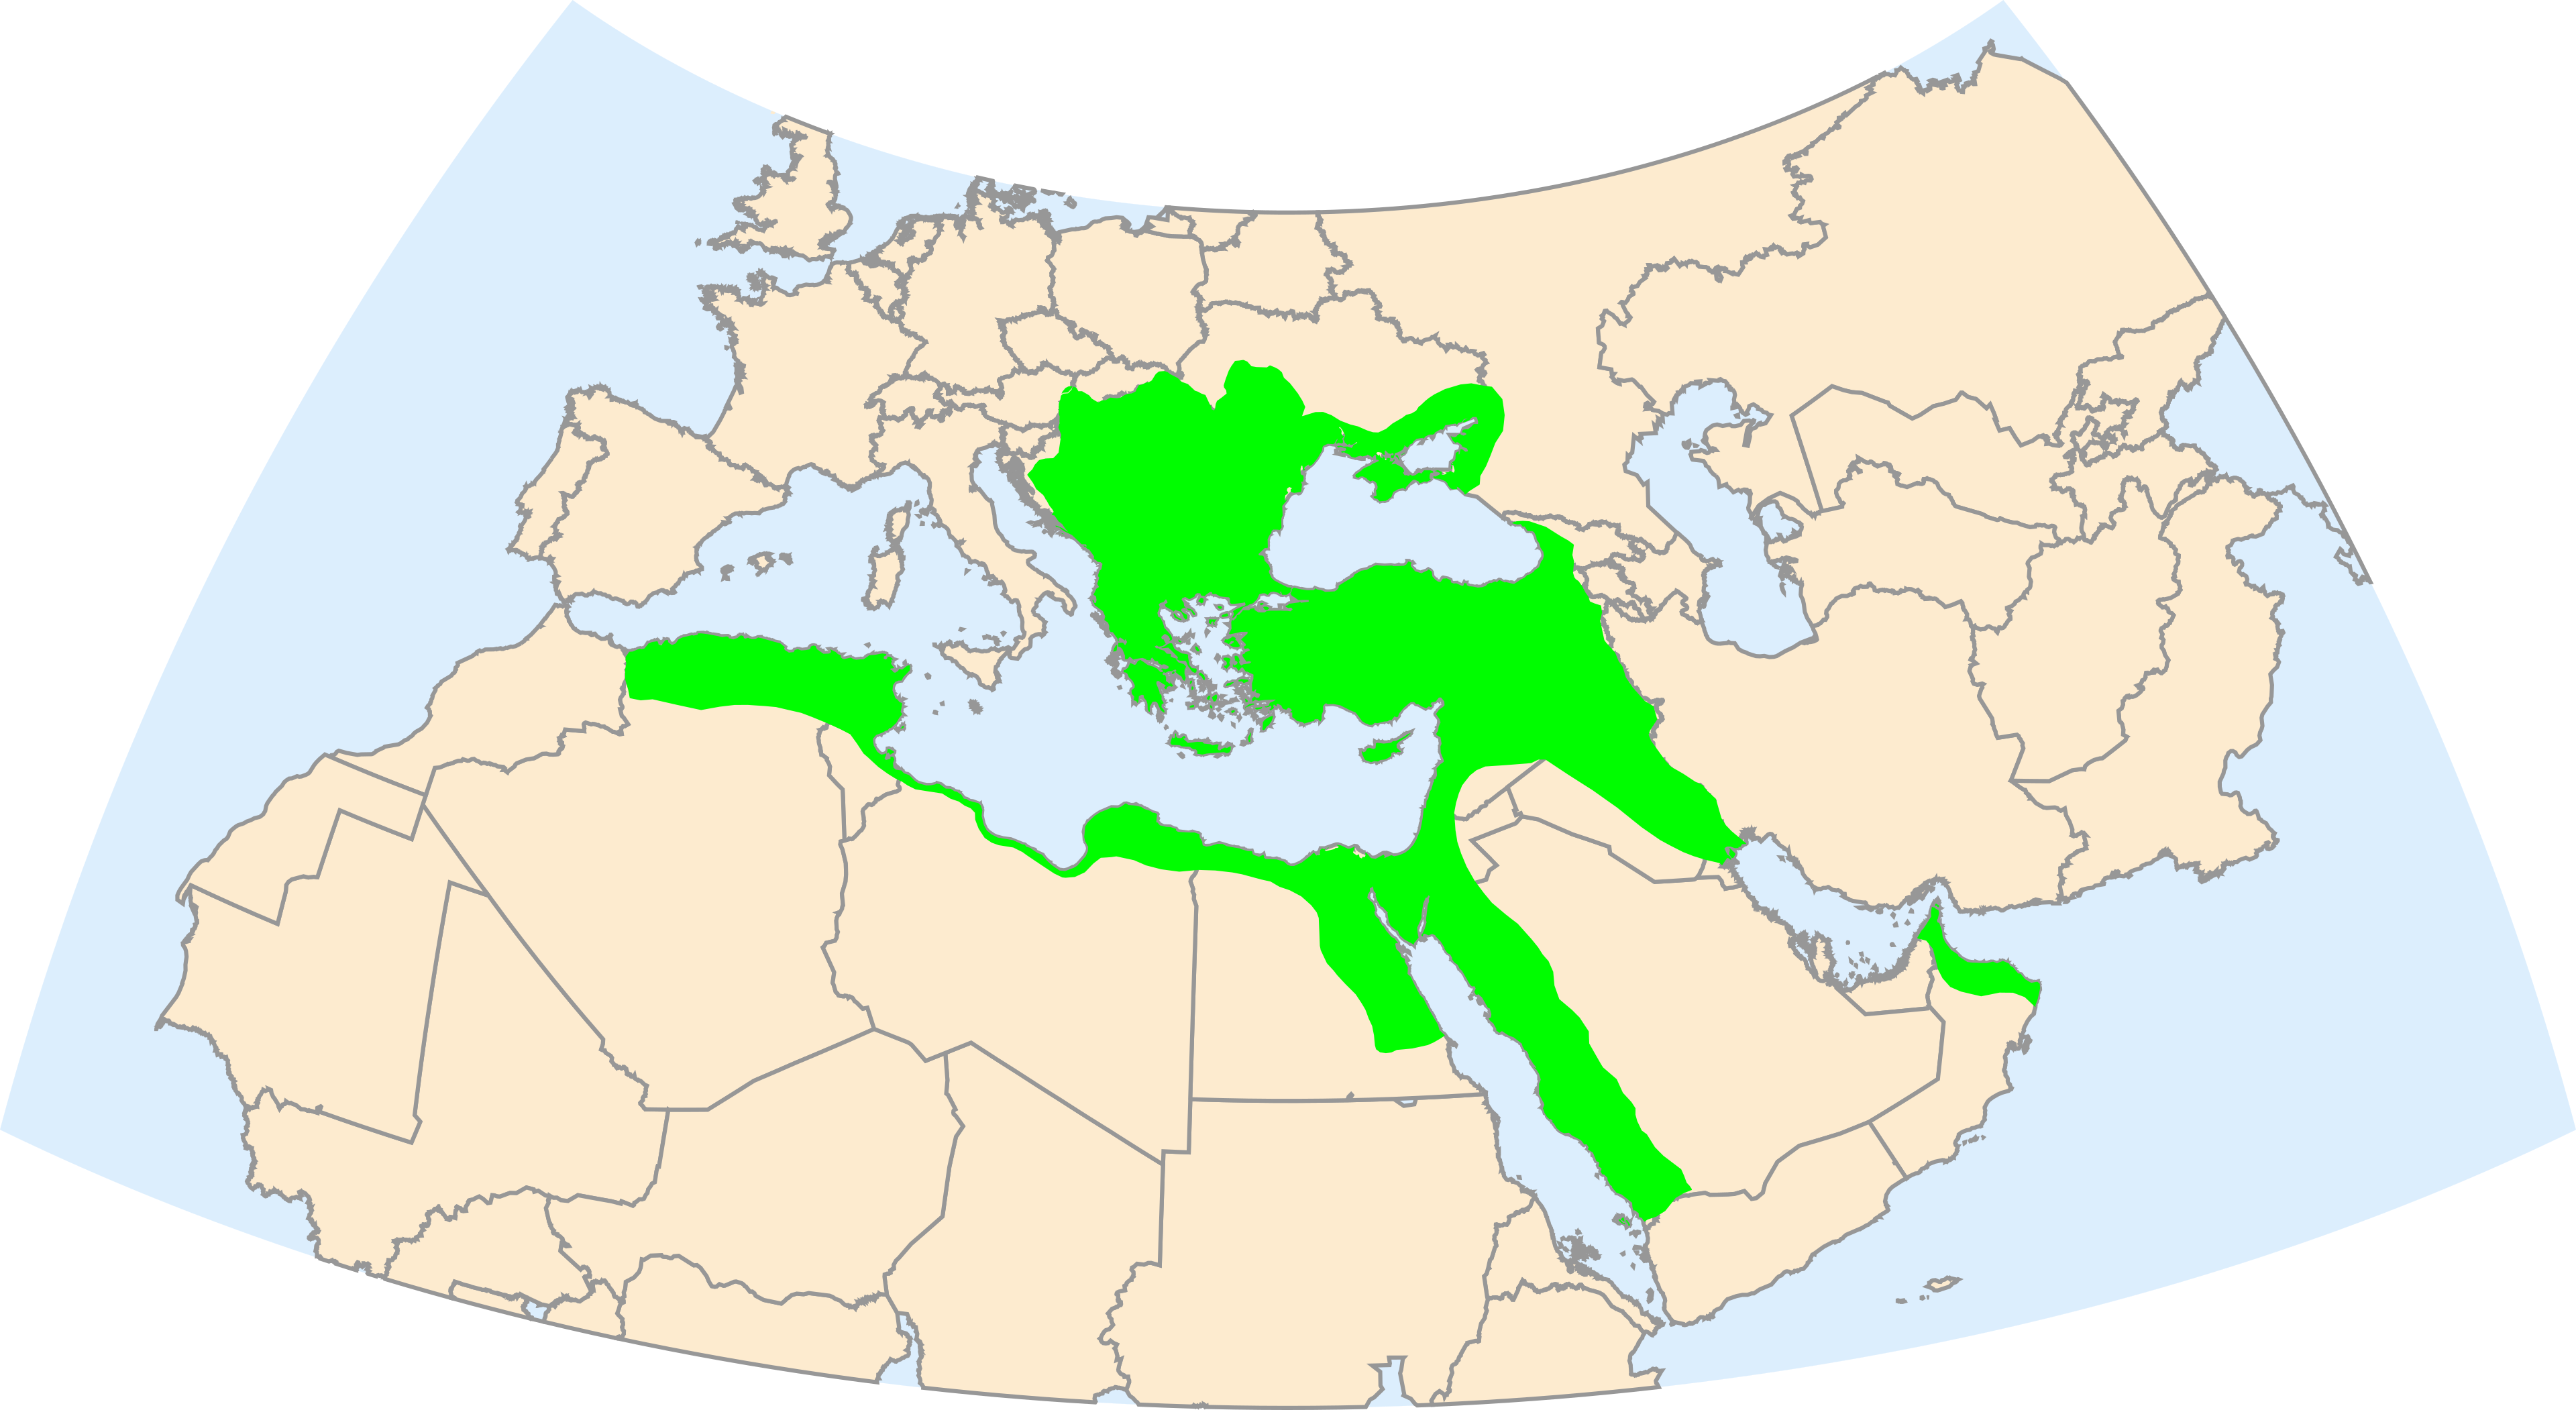
\includegraphics[width=1.4\textwidth]{1683OttomanEmpire.png}
			\end{figure}
			
	\end{columns}
\end{frame}

\section{Early 20\inst{th} Century}
\begin{frame}{Early 20\inst{th} Century}
	\begin{columns}
		\column{0.3\textwidth}
			\begin{enumerate}
				\item Orient Express
				\item World War I
			\end{enumerate}
		\column{0.7\textwidth}
			\vspace{-0.2\textheight}
			\begin{figure}[ht]
				\centering
				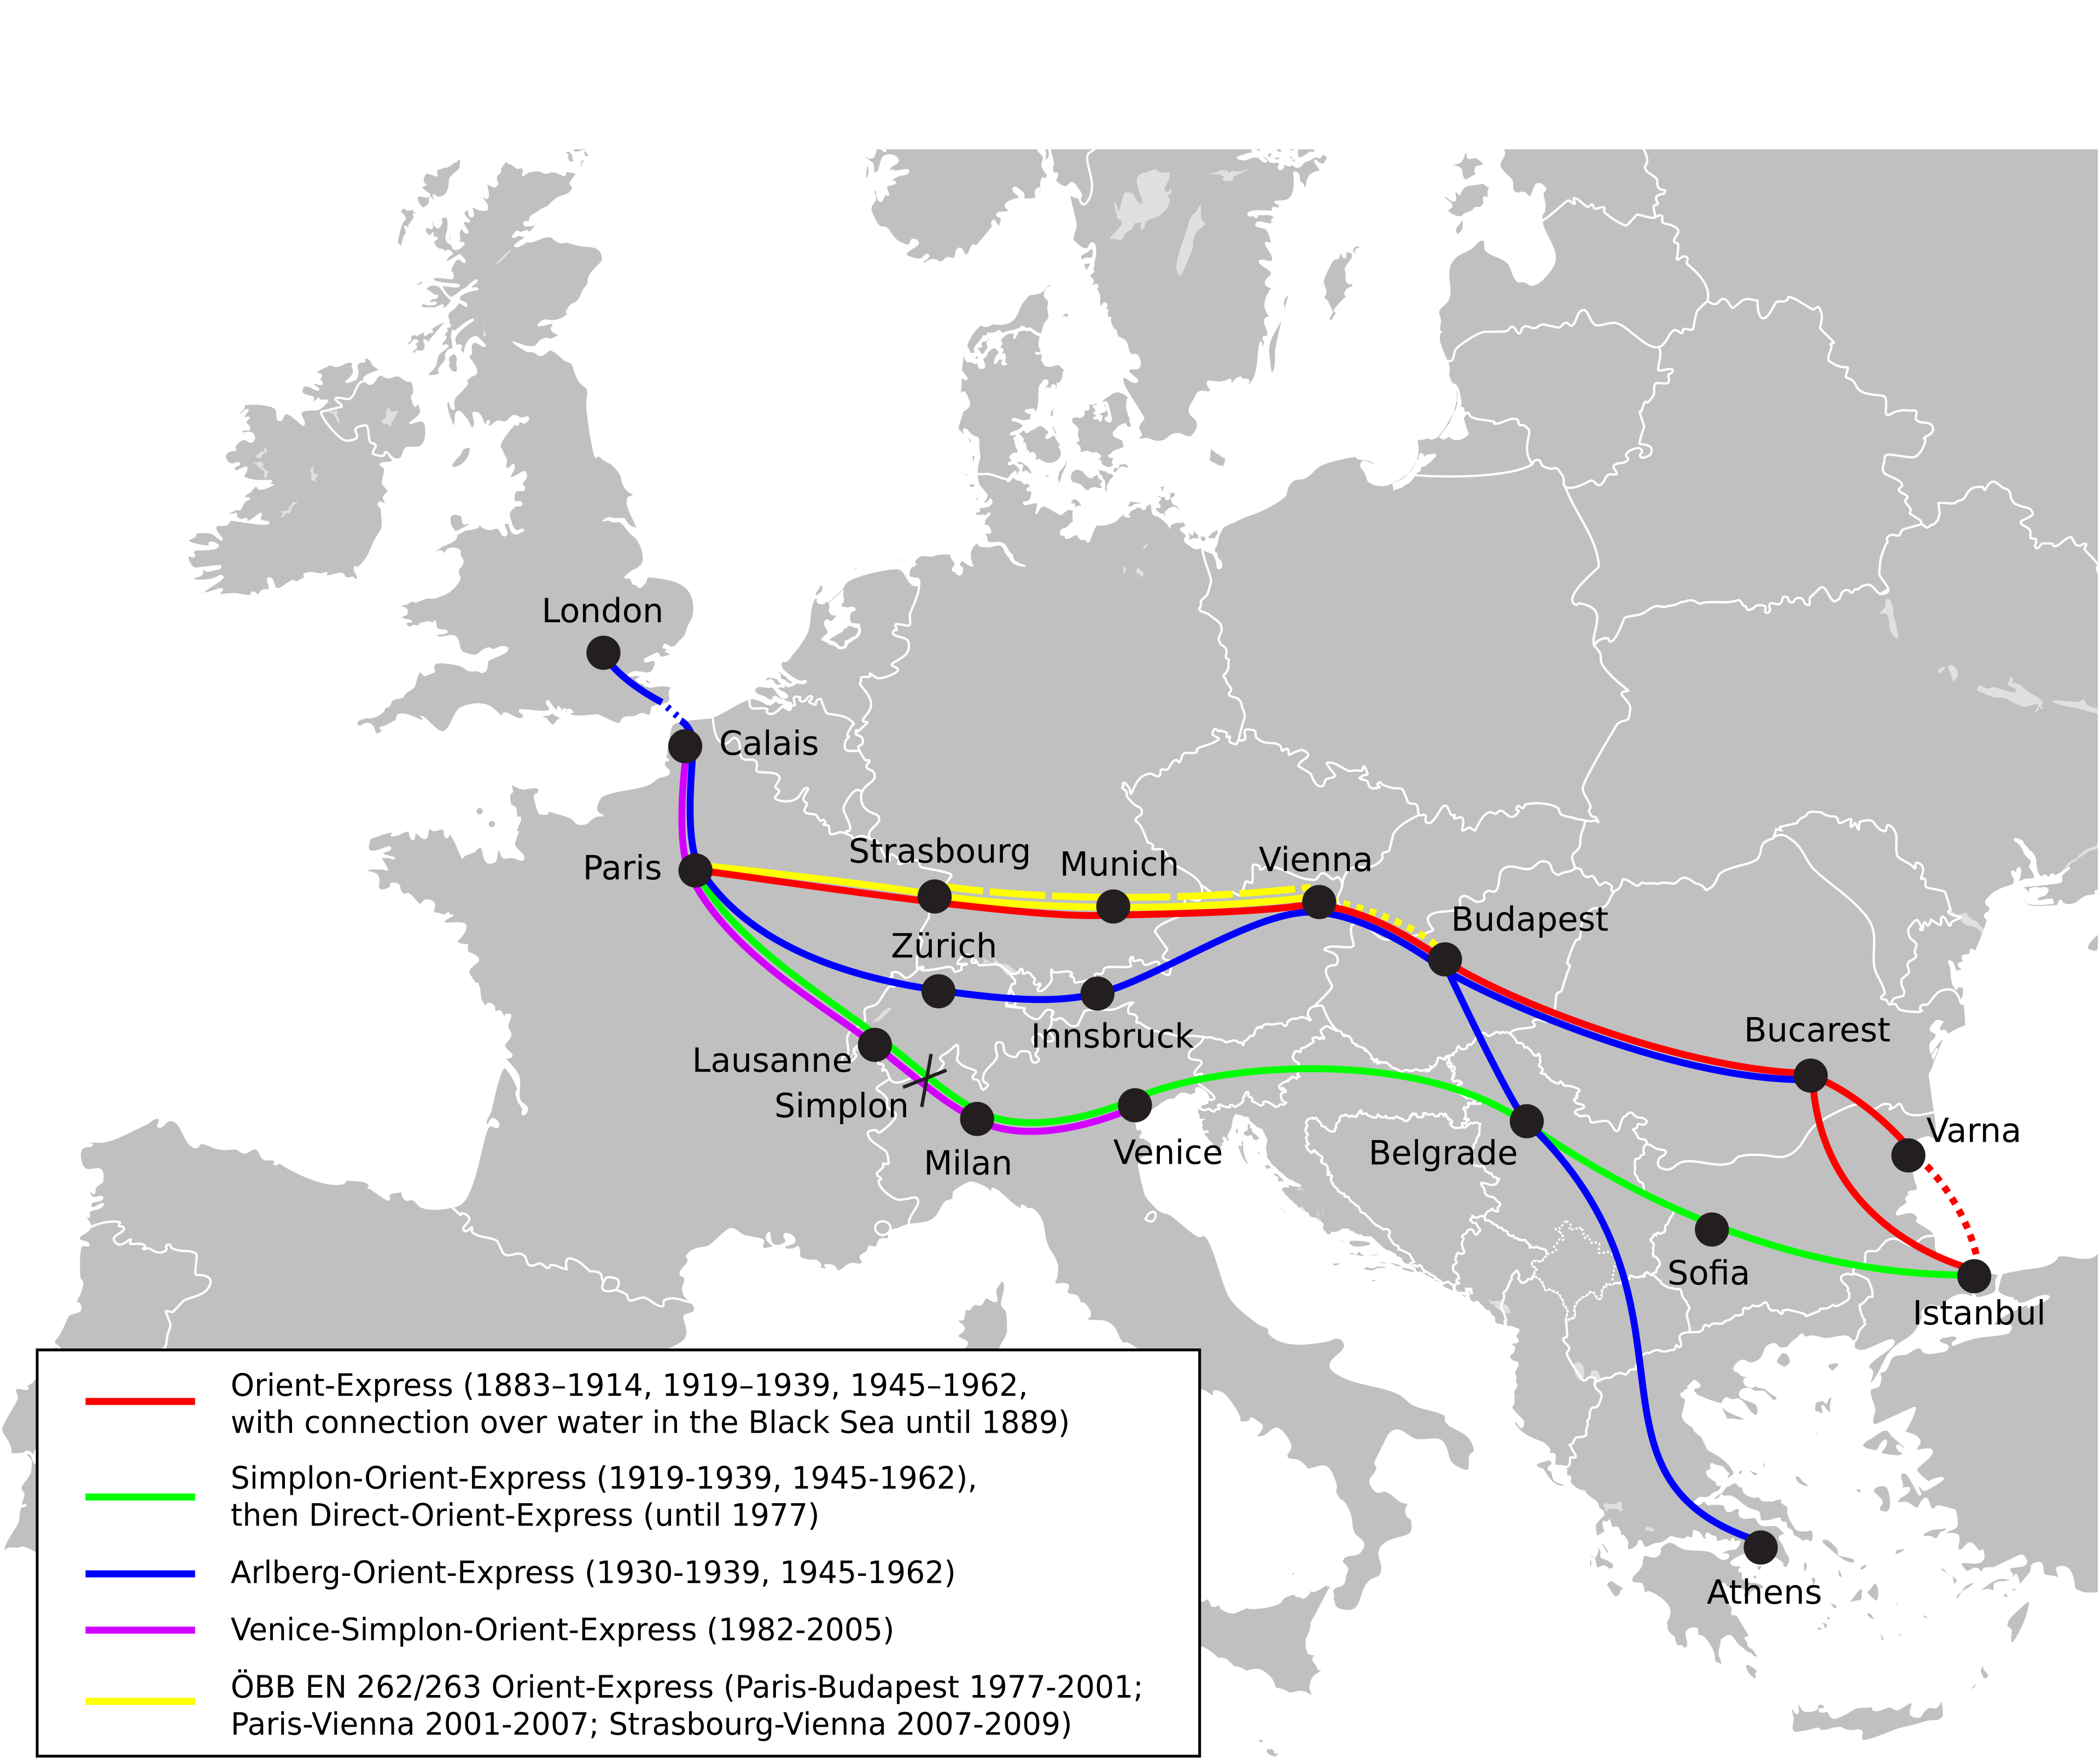
\includegraphics[width=1.1\textwidth]{oxpress.png}
			\end{figure}
	\end{columns}
\end{frame}

\section{Late 20\inst{th} Century}
\begin{frame}{Late 20\inst{th} Century}
	\begin{enumerate}
		\item Family Reunification (1974)
		\item West Berlin Labor (1969-1989)
		\item Greece Trap (1950's)
	\end{enumerate}
\end{frame}

\section{The Third Millenium}
\begin{frame}{The Third Millenium}
	\begin{columns}
		\column{0.4\textwidth}
			\begin{enumerate}
				\item Israel/Lebanon War
				\item Syrian Civil War
				\item Turkish \emph{coup d'\`{e}tat}
			\end{enumerate}
		
		\column{0.6\textwidth}
		\begin{table}[ht]
			\centering
			\begin{tabular}{|c|c|}
				\hline
				\bf{Country} & \bf{Turkish Citizens in Residence}\\
				\hhline
				Germany & 2,700,000\\
				\hline
				France & 820,000 (2014 estimate)\\
				\hline
				Netherlands & 372,728\\
				\hline
				United States & 250,000\\
				\hline
				Austria & 159,958\\
				\hline
			\end{tabular}
			\caption{Turkish Citizens Abroad}
		\end{table}
	\end{columns}
\end{frame}

\section*{Questions}
\begin{frame}{Questions}
\centering
\vcenter
	\Huge?
\end{frame}

\section*{References}
\begin{frame}{References}
	\begin{itemize}
		\item UN Database (UNDat)
		\item Nathans, Eli (2004), The Politics of Citizenship in Germany: Ethnicity, Utility and Nationalism, 
		\item Findley, Carter (2005), The Turks in World History, Oxford Universit
		\item  "Turkish migrants grieve for Beirut from exile". Today's Zaman
	\end{itemize}
	
\end{frame}

\end{document}
